\section{Einführung}

\subsection{Prinzip}
Die FM Synthese ist eine für die Musikwelt sehr wichtige Anwendung der Frequenzmodulation, welche bereits aus der Nachrichtentechnik bekannt ist. Generell wird dabei die Frequenz eines Trägersignals durch ein weiteres Modulationssignal verändert, die Amplitude bleibt jedoch unangetastet. In der Nachrichtentechnik können durch die unterschiedlichen Frequenzen im modulierten Trägersignal dadurch Informationen übertragen werden. 

Die momentane Amplitude des modulierten Signals lässt sich durch folgende Formel beschreiben:

\[
e(t) = A\sin(\alpha t + I\sin(\beta t)) 
\]

Bei der äußeren Sinusfunktion handelt es sich um das Trägersignal, welches in seiner Frequenz durch das Modulationssignal (Innerer Sinus) moduliert wird.


Abbildung \ref{fig:vergleichSignale} veranschaulicht die Frequenzmodulation eines Signals durch ein zweites Signal.

\begin{figure} [ht]
\centering
  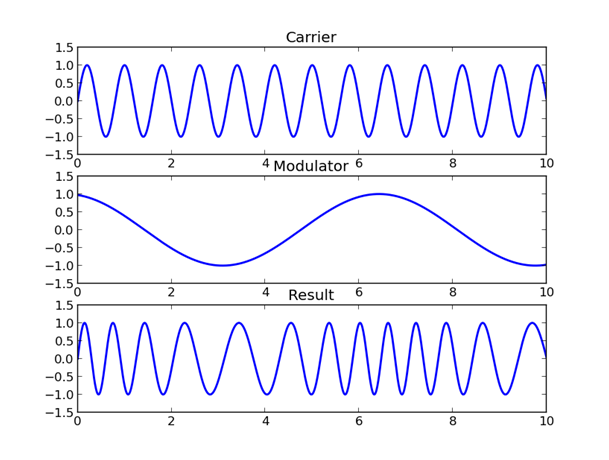
\includegraphics[width=0.95\textwidth]{Signalbeispiel.png}
\caption{Vergleich Träger/Modulator}
\label{fig:vergleichSignale}
Quelle: \url{http://www.gcat.org.uk/blog/wp-content/uploads/2013/01/synth3_4.png}
\end{figure}

Wie man gut erkennen kann, wird die Frequenz des Trägers bei hoher Amplitude des Modulators größer, bei negativer Amplitude dagegen kleiner. Ist die Amplitude des Modulators gleich 0, so wird das Trägersignal nicht moduliert.

Die Frequenzmodulationssynthese ist in ihren Grundzügen recht einfach zu verstehen und man kann mit geringem Aufwand bereits sehr komplexe, wenn auch oft unkontrollierbare Signale mit komplexen Klangspektren (bzw. Frequenzspektren) erzeugen. Wie sich im Folgenden jedoch noch herausstellen wird, ist es dagegen sehr schwierig und erfordert viel Zeit und Aufwand, durch die FM-Synthese gezielt Signale zu erzeugen und diese zu kontrollieren. Eine Möglichkeit zur Erzeugung komplexer Klangspektren ist es, den Modulationsindex innerhalb des Trägersignals zeitabhängig zu machen. Dieses Verfahren wird im Kapitel X näher erläutert.

Praktisch gesehen kann die Frequenzmodulations-Synthese dazu verwendet werden, um zum Einen Klangbilder echter Instrumente digital nachzubilden, jedoch auch, um ganz neue Töne zu erzeugen, die so in der realen Welt nicht vorkommen. Im Folgenden sind einige Beispiele von durch FM-Synthese erzeugten Signalen zu sehen.

\subsection{Beispiel (Sound \& Visualisierung)}
\subsection{Geschichte der FM-Synthese}
Die Grundlegende Technik hinter der FM-Synthese stammt, wie bereits erwähnt, aus der Nachrichtentechnik. Dort wird das Verfahren Frequenzmodulation genannt. Im Jahre 1967 entdeckte Prof. Dr. John Chowning eine neue Eigenschaft dieses Verfahren. Während er mit unterschiedlichen Modulationsfrequenzen experimentierte und dabei verschiedene Vibrato erzeugte (unter Vibrato versteht man einen schwingenden Ton, d.h. eine pulsierende Änderung des Tons), verschwand der Vibrato plötzlich bei höheren Modulationsfrequenzen und Obertöne wurden hörbar, die sich vom eigentlichen Trägersignal abhebten.

Chowning selbst war sehr erstaunt über die entstandenen Töne. Da er seiner Meinung nach der erste Mensch war, der diese Töne durch einen Computer erzeugt hatte, dachte er: 

``I was aware that I was probably the first person to ever hear these sounds, that what I was hearing was something musical that had probably never been heard by anyone before — at least, not by anyone on this planet.'' - John Chowning, 1967

Es dauerte weitere 3 Jahre, bis Chowning die mathematischen Zusammenhänge hinter seiner Entdeckung vollständig ergründet hatte. Bis dahin war er außerdem bereits in der Lage, verschiedene Instrumente wie Trommeln oder Blasinstrumente nachzubilden. Da Chowning selbst leidenschaftlicher Komponist war, veröffentlichte er im Jahre 1971 sein erstes, rein durch FM-Synthese generiertes Stück mit dem namen ``Sabelithe''. 
 
\begin{figure} [ht]
\centering
  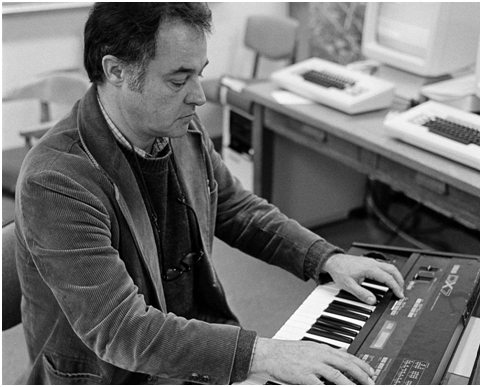
\includegraphics[width=0.95\textwidth]{chowning_CCRMA.png}
\caption{John Chowning am CCRMA}
Quelle: \url{http://arts.mit.edu/wp-content/uploads/2014/07/ChowningYamaha.jpg}
\end{figure}
 
Da Prof. Chowning seine Entdeckung nicht auf eigenes Risiko hin patentieren lassen wollte, lies er dies durch das OTL (Stanford Office of Technology Licensing) durchführen. Er selbst sagte dazu:

``I didn’t want to deal with lawyers — I wanted to do my music. I didn’t care about the money as much as I cared for my compositions. It was natural for me to say, `Please take it.' ''

 Seine neue Entdeckung war jedoch zu Beginn nicht sehr angesehen und auch viele der Firmen, welchen das neue Patent angeboten wurde, wussten nichts damit anzufangen und lehnten ab. Erst im Jahr 1974, als ein junger Ingeneur namens Kazukiyo Ishimura von der Firma Yamaha, zu einer Vorstellung des Verfahren geschickt wurde, erkannte dieser binnen wenigen Minuten das Potenzial hinter dieser neuen Anwendung der Frequentmodulation und Yamaha Lizensierte das Verfahren im gleichen Jahr. Ishimura wurde später Chef des Yamaha Konzerns. 

Im Jahr 1975, nach einiger Zeit Abwesenheit von Stanford, kehrte Chowning dorthin zurück und gründete zusammen mit einigen seiner Kollegen das CCRMA (Center for Computer Research in Music and Acoustics), welches sich auf Computermusik spezialisiert hat.
Nachdem Yamaha die Technik der FM-Synthese lizenziert hatte, brachten die Firma nach einem Prototypen im Jahre 1980 den ersten digitalen FM Synthesizer GS1 und zwei Jahre später mit dem GS2 eine kleinere und handlichere Version des GS1 heraus. Beide Geräte kosteten um die 12.000 \textdollar und waren deshalb nur für ausgewählte Musiker gedacht. Der Durchbruch gelang im Jahre 1983 mit dem DX7. Dieser konnte parallel 16 Stimmen verarbeiten und kostete ca. 2000 \textdollar. Preislich ähnliche und damals übliche analoge subtraktive Synthesizer konnten lediglich 4 Stimmen verarbeiten. Ein Bild des DX7 ist in Abbildung \ref{fig:dx7} zu sehen.

 \begin{figure} [ht]
\centering
  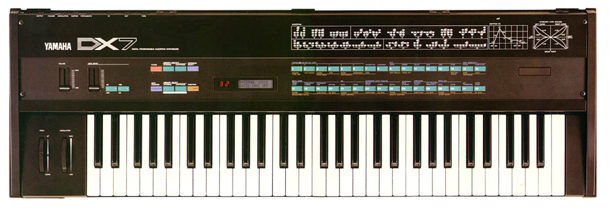
\includegraphics[width=0.95\textwidth]{dx7.png}
\caption{Yamaha DX7}
\label{fig:dx7}
Quelle: \url{http://www.electricdruid.net/images/interface/larger/YamahaDX7.jpg}
\end{figure}

Durch den großen Erfolg des DX7 konnte Yamaha in den nachfolgenden Jahren viele Weiterentwicklungen auf den Markt bringen. In den Jahren 1983 bis 1989 brachte Yamaha über 20 weitere digitale Synthesizer heraus. Über die Zeit wurden jedoch andere Syntheseverfahren günstiger und für den Markt besser geeignet, weshalb Yamaha 1990 mit dem SY77 Synthesizer ein Gerät entwickelte, das FM-Synthese und ein anderes digitales Klangsyntheseverfahren namens Sampling in einem vereinte. 

Ab Mitte der 1990er wurden Personal Computer leistungsfähig genug, um Synthesizer ohne Verzögerung durch eine Midi Tastatur ansprechbar zu machen. Heutzutage findet digitale Audioverarbeitung nahezu ausschließlich softwareseitig statt, weshalb Hardwaresynthesizer wie der DX7 an Bedeutung verloren haben. Speziell dieser wurde jedoch durch die Firma Native Instruments in Form des FM7 und dessen Weiterentwicklung, dem FM8, in Software nachgebaut und findet heute noch Verwendung. Auch ist der DX7 heute bei Nostalgikern noch sehr beliebt.

